\documentclass{article}
\usepackage{graphicx} % Required for inserting images

\title{Problem Set 6}
\author{adam spohn}
\date{March 2024}

\begin{document}

\maketitle

\section{Data Cleaning}

For this problem set I used the same data that I collected in the last problem set. I did a bit of data cleaning in the last one already so I left those steps in. For the data reference that one had all the wrong column names, some columns that came in were useless, on one column was twice as long with every odd row being data from some other area that I did not recognize or need. For this I got rid of the useless columns, renamed all the columns, and got red of every odd numbered row of the "FIP" column. I also added some NA's to make the columns equal length, since some of them stole some extra rows. Additionally, I wanted to put labels on my plots, but I did not want entire team names as labels so I added in team name abbreviations. I also had to change the variables to numerics in order to work with them. 

For the FRED data I had to do next to no data cleaning, it was pretty well already to work with, I just fixed the issue from the last problem set so that the API key is coming from my .Renviron file now.

\begin{figure}
    \centering
    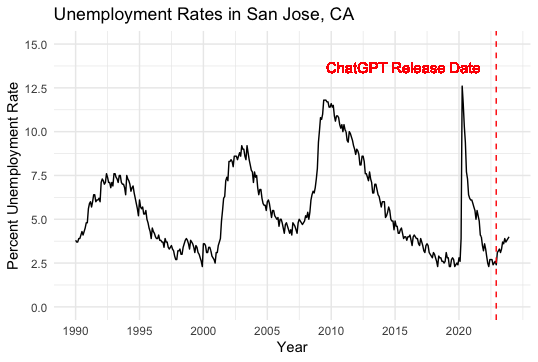
\includegraphics[width=0.8\linewidth]{PS6a_Spohn.png}
    \caption{San Jose, CA, Unemployment, and ChatGPT release}
\end{figure}


\begin{figure}
    \centering
    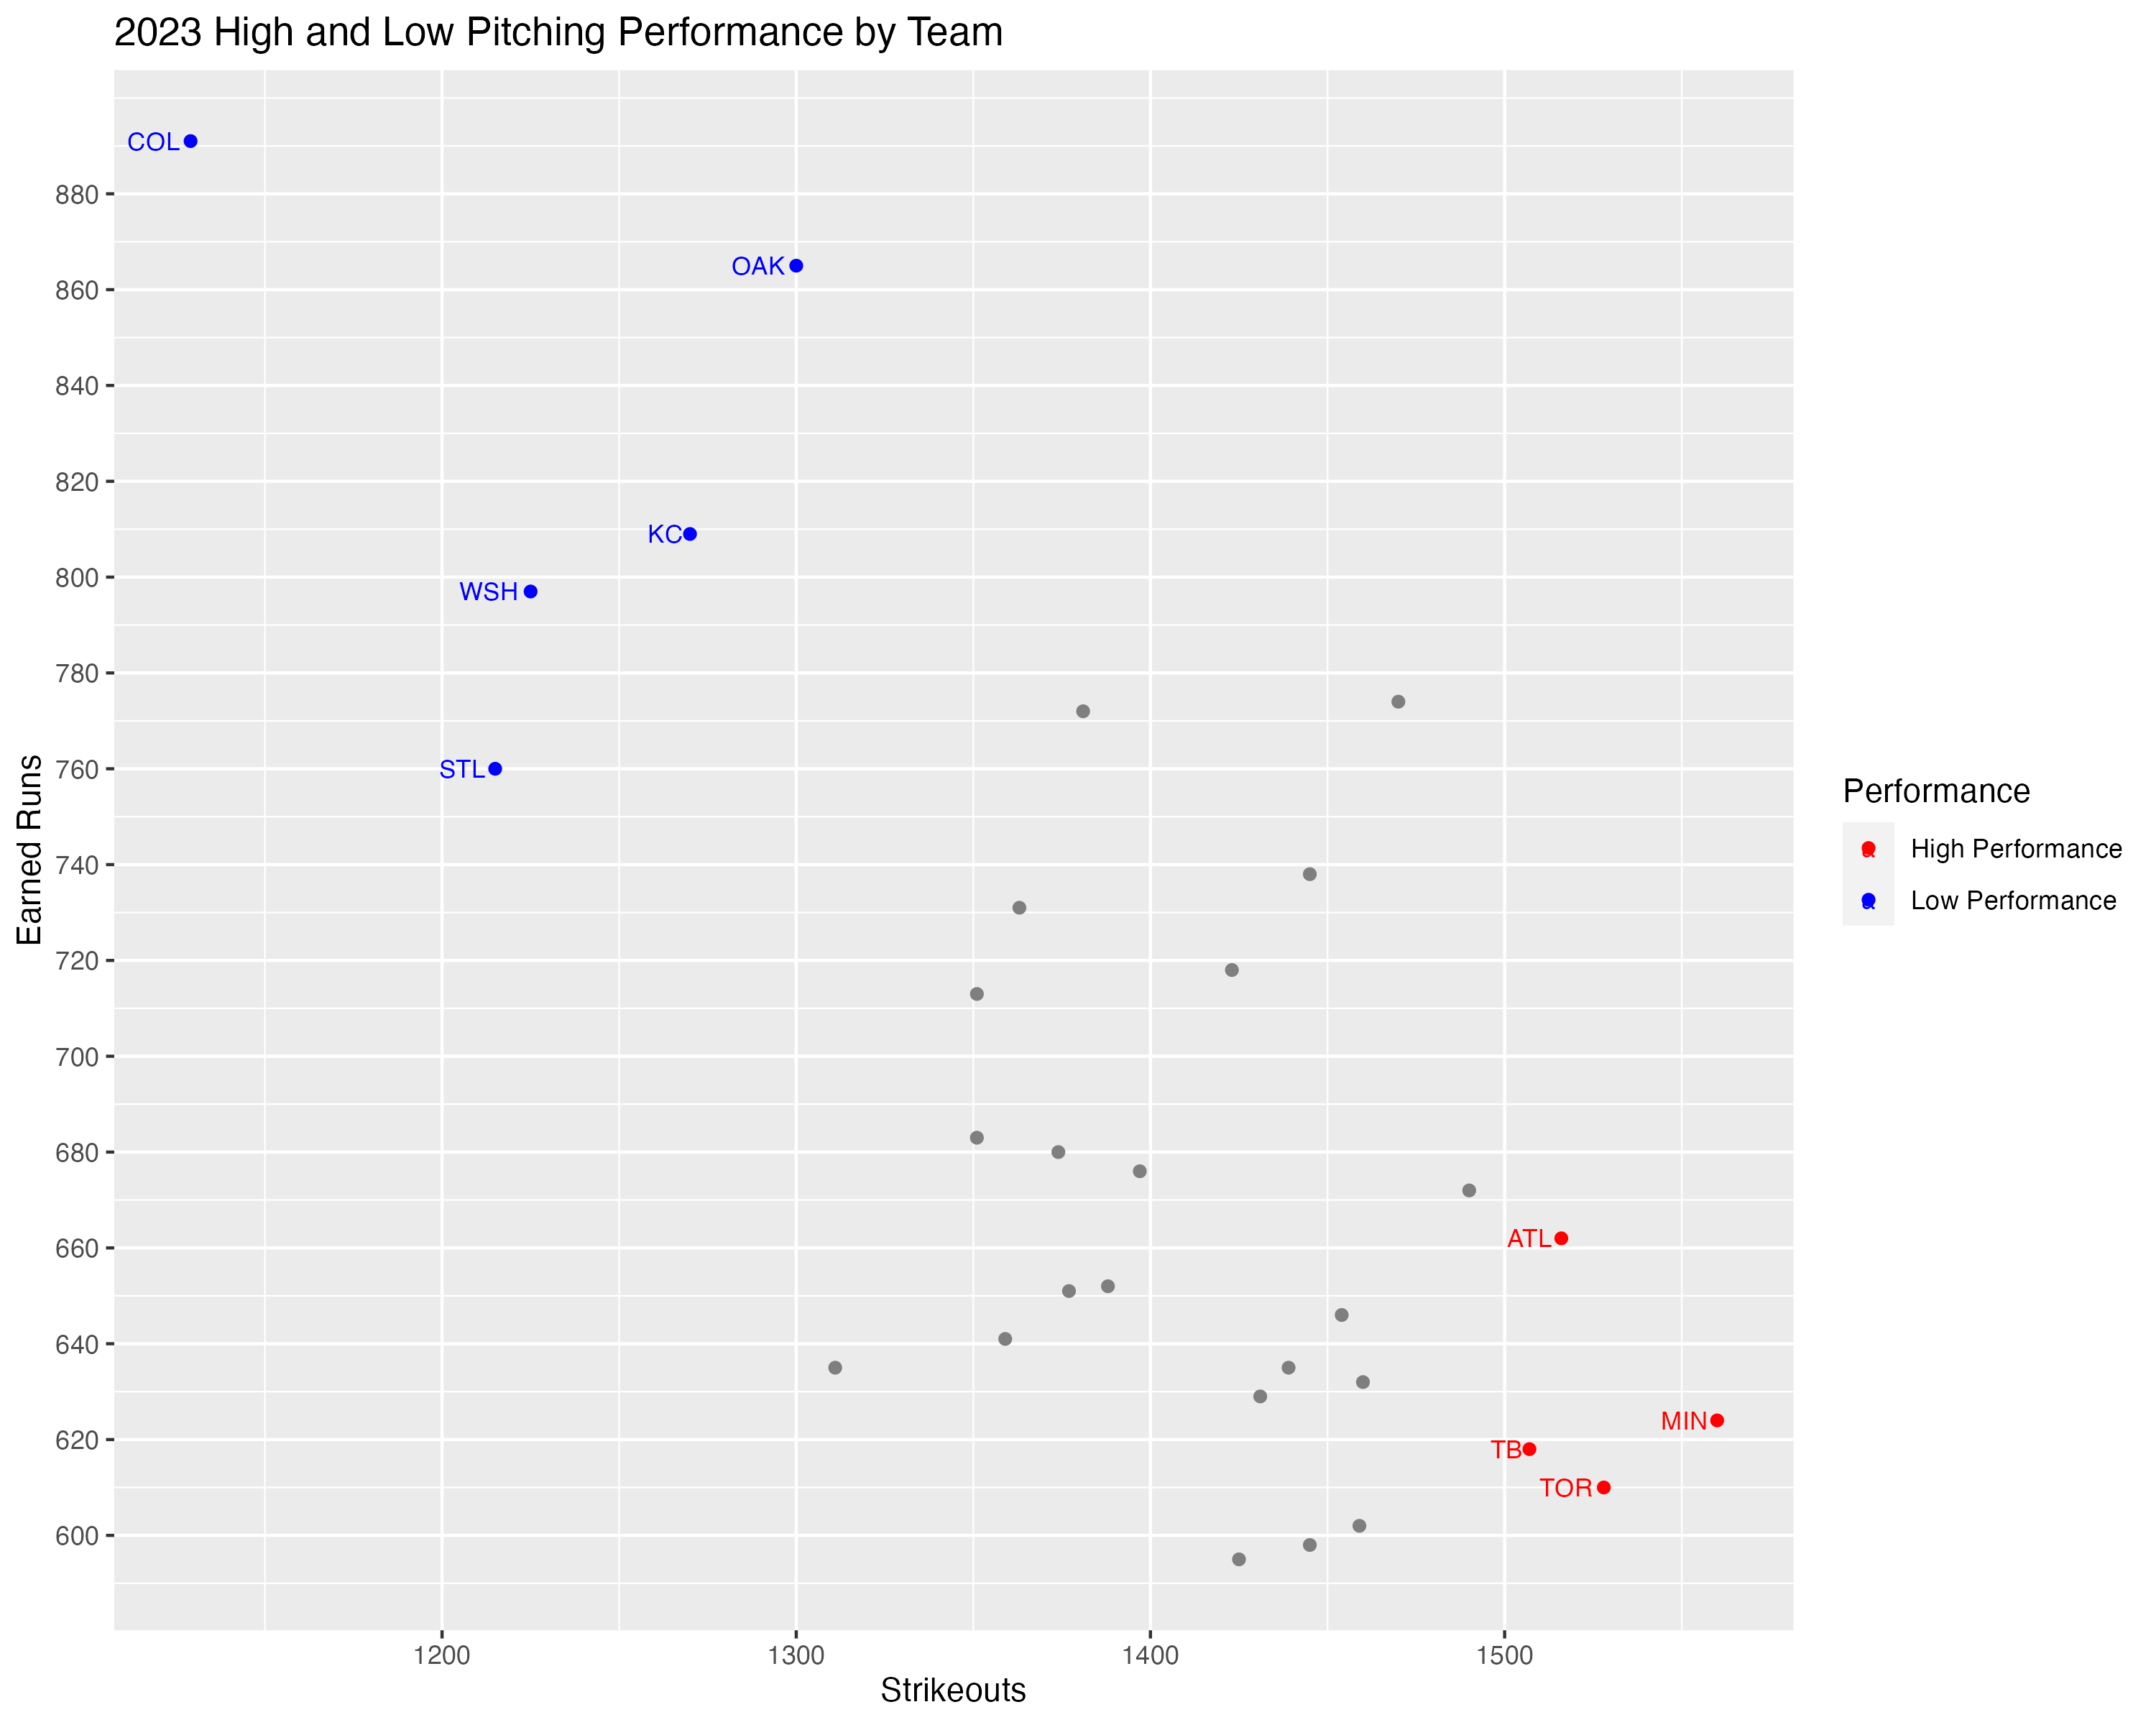
\includegraphics[width=0.8\linewidth]{PS6b_Spohn.png}
    \caption{Measure of MLB team pitching using strike outs and earned runs}
\end{figure}

\begin{figure}
    \centering
    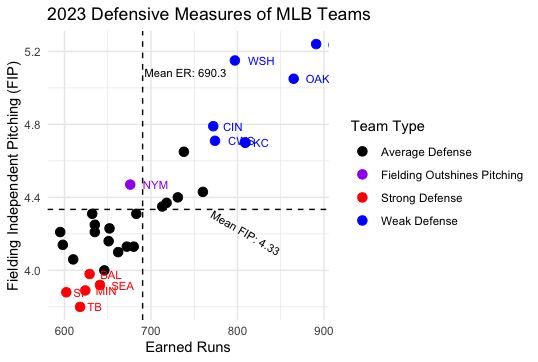
\includegraphics[width=0.8\linewidth]{PS6c_Spohn.png}
    \caption{Measure of MLB team defense using FIP and earned runs}
\end{figure}

\section{Graph Explanations}
Figure 1 is a graph of the release date of ChatGPT over the graph of an unemployment time series in San Jose, CA. The idea of this graph is that we can look to see if employment factors had any reaction to the release of ChatGPT. I focused on San Jose, because I thought it would be a good representation of Silicon Valley, somewhere that I thought might be particularly affected by ChatGPT, one way or another. I do not think this graph can answer this question on its own, and the time following the release is very small, though unemployment did increase following its release. This can of course just be a coincedence.

Figure 2 tries to measure at the team level pitching effectiveness in the MLB. It does so by using a scatter plot looking at strike outs and earned runs. Only the teams with a high strike outs and low earned runs, and vice versa, are labeled. This is both to reduce clutter that would reduce visibility, and just focus on pointing out who the best and worst teams were, or the outliers. 

Figure 3 is similar to figure 2, though this time I tried to make it more about general defense rather than just pitching, and I believe two variables measured, FIP and earned runs can sort of do so. Since different levels of FIP or earned runs could maybe mean good or bad pitching, or maybe good or bad fielding, I built quadrants for this one. I did so by making the quadrant dividing lines the league averages for FIP and earned runs. Not many teams Appeared in quadrant 2 or 4. Teams appearing in poor FIP but good earned runs I interpreted as having poor pitcing, but fielding that outshined that fact. Outside of this I again highlighted and only labeled teams deeper in the other two quadrants. That way this plot shows you the best, worst, and unique defenses in the MLB, theoretically. 

\end{document}
